\section{Application}

A typical application of Catalan Numbers is the number of ways from $(0, 0)$ to $(n, n)$ in a $n \times n$ grid without crossing the line $y = x-1$ (\ref*{fig:basic}).

we can explain both the general formula and the recurrence formula in the context of this application. The general formula is used to calculate the number of ways to reach $(n, n)$ from $(0, 0)$ in a $n \times n$ grid without crossing the line $y = x-1$. The recurrence formula is used to calculate the number of ways to reach $(n, n)$ from $(0, 0)$ in a $n \times n$ grid without crossing the line $y = x-1$ by using the number of ways to reach $(n-1, n-1)$ from $(0, 0)$ in a $(n-1) \times (n-1)$ grid without crossing the line $y = x-1$.

It's clear that the number of ways to reach $(n, n)$ from $(0, 0)$ in a $n \times n$ grid without crossing the line $y = x-1$ is equal to the number of ways to reach $(n, n)$ from $(0, 0)$ without constraints minus the number of ways to reach $(n, n)$ from $(0, 0)$ in a $n \times n$ grid without crossing the line $y = x-1$. 
But we can always do a symmetry transformation with respect to the line $y = x-1$ as Figure~\ref{fig:symmetry} shows. Then
\[
    C_n = \binom{2n}{n} - \binom{2n}{n-1} = \frac{1}{n+1}\binom{2n}{n}.
\]

\begin{multicols}{2}
    \begin{figure}[H]
        \centering
        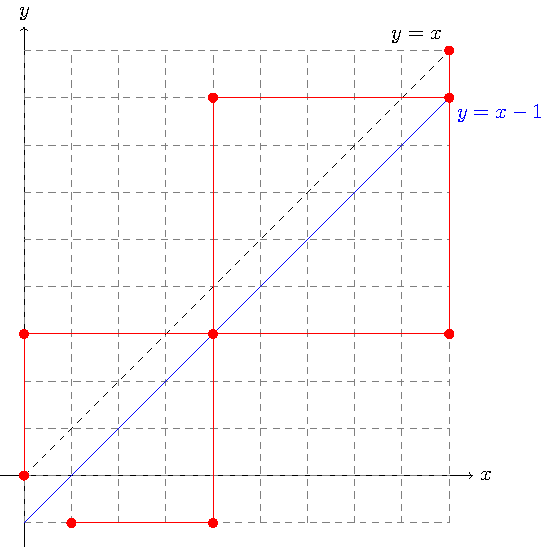
\includegraphics[width=0.9\columnwidth]{figures/symmetry.pdf}
        \caption{general Formula}\label{fig:symmetry}
    \end{figure}
    \begin{figure}[H]
        \centering
        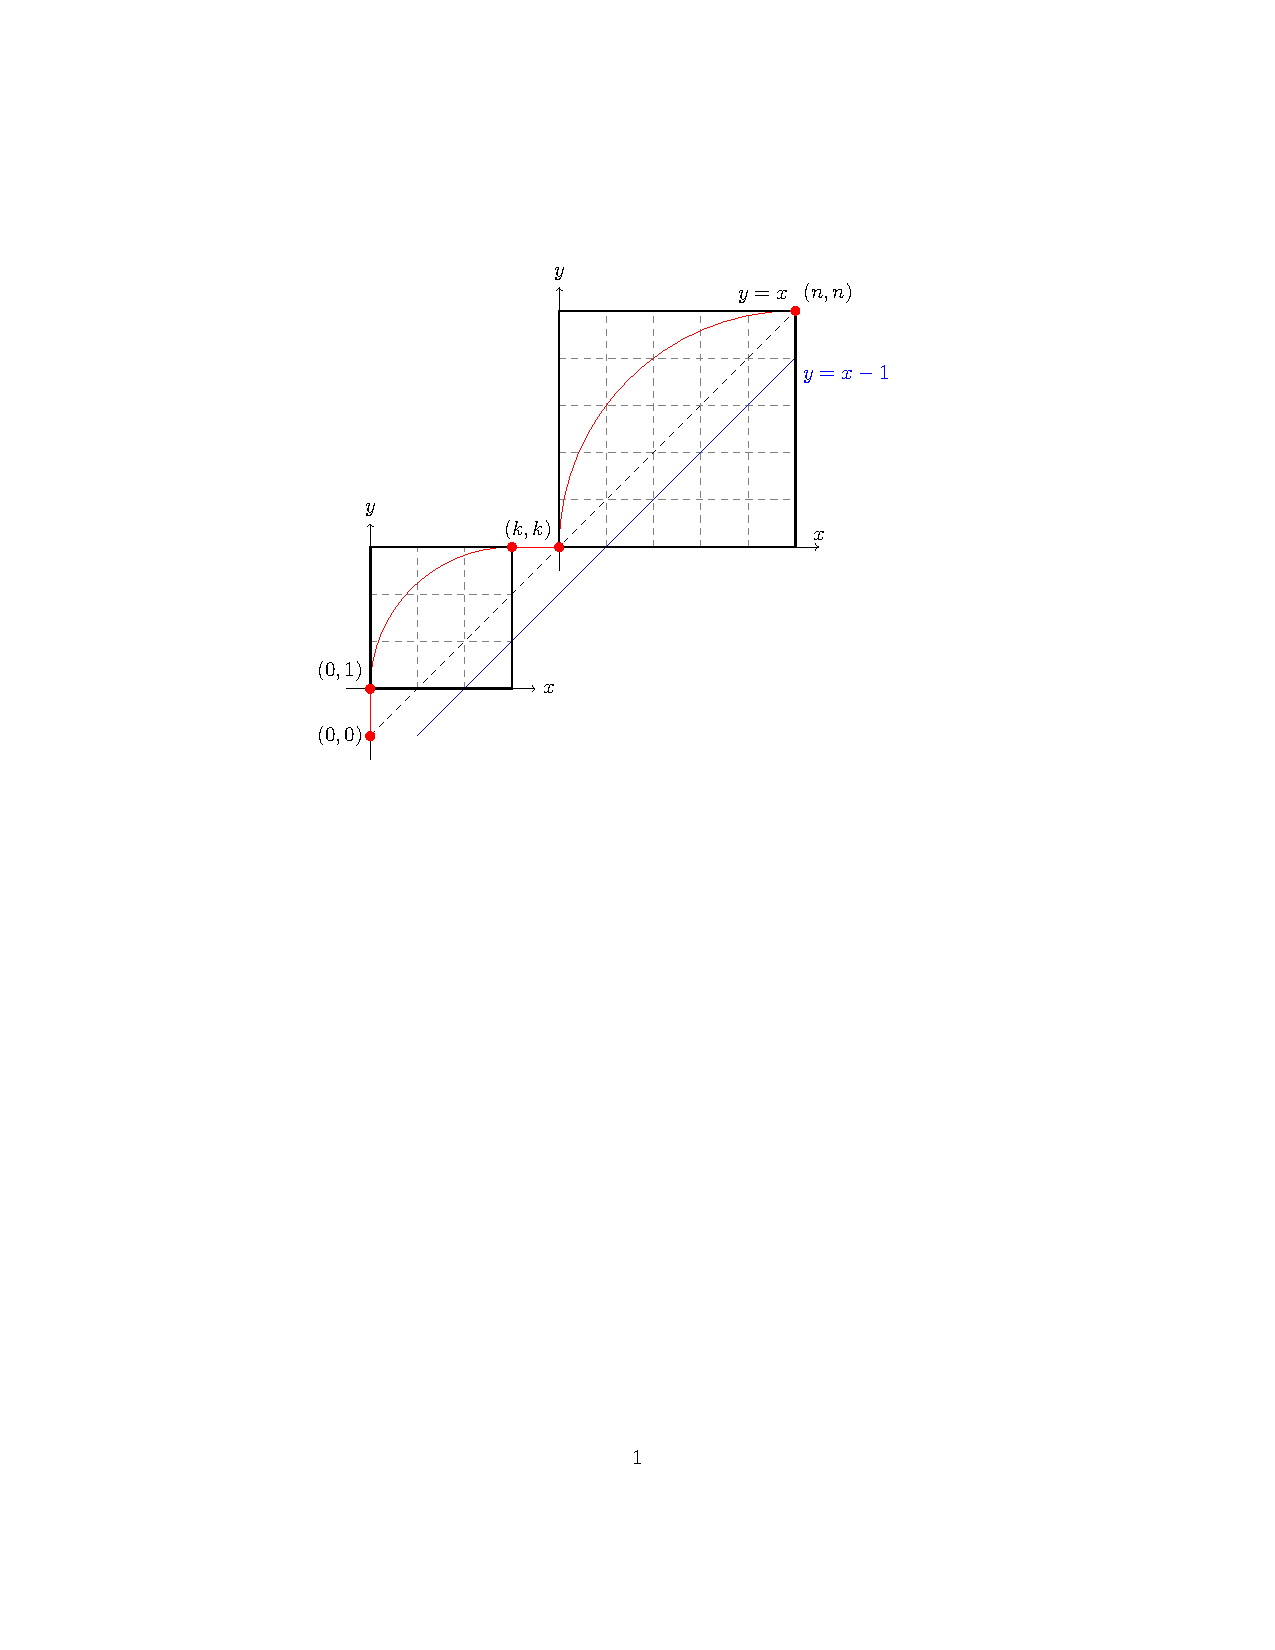
\includegraphics[width=\columnwidth]{figures/recurrence.pdf}
        \caption{recurrence Formula}\label{fig:recurrence}
    \end{figure}
\end{multicols}

On the other hand, suppose we firstly touch $y=x$ at point $(k,k)$, then we can divide the path into two parts: the first part is from $(0,0)$ to $(k,k)$ (i.e. $(0,1)\to(k-1,k)$), and the second part is from $(k,k)$ to $(n,n)$. By principle of multiplication, we can traverse the first part in $C_k$ ways and the second part in $C_{n-1-k}$ ways. Therefore,
\[
    C_n = \sum_{k=0}^{n-1} C_kC_{n-1-k}.
\]